\section{Results and Discussion}
% Structure with subsections
% Use of figures/tables (max. 5)
% General description of the results
\subsection{Differentially Expressed Genes and Network Creation}

Under the chosen thresholds discussed in section \ref{sec:methods-deg}, 908 genes were found to be differentially expressed. Around half (495) are up-regulated, and the remaining 413 are down-regulated. STRING could query 828 of them; using other ID types did not change this. After querying the additional EDS-related genes, the resulting network consists of 847 genes and 6129 connections.

The position of the known EDS genes in the network is, on average, more central than expected by chance based on degree, clustering coefficient, betweenness centrality and closeness centrality, supporting the close relationship between hEDS and other EDS types.

\subsection{Enrichment analysis and clustering}

GO-enrichment is performed on the DEGs to acquire an overview of over-represented molecular functions, biological processes and cellular components. In contrast to later results, which include the known EDS genes, this analysis is performed purely on the differentially expressed genes.

Biological processes over-represented in the DEGs include cell-cycle regulation, signalling and transition, nucleosome assembly and organisation and protein-DNA assembly and organisation.  Cellular components affected are the nucleosome (GO:0000786), the chromosomal region (GO:0098687 and GO:0000775), the protein-DNA complex (GO:0032993) and the collagen-containing extracellular matrix (ECM) (GO:0062023). Over-representation analysis for the molecular function is less meaningfull on a large network. Still, three terms are related to a significantly higher number of genes than the rest: The structural constituent of chromatin (GO:0030527), protein heterodimerization activity (GO:0046982) and extracellular matrix structural constituent (GO:0005201).

[TODO: Do i want to look at Pathways? lupus and alcoholism maybe not that interesting, but Cell cycle?]

[TODO: Analysis]

\subsubsection{MCODE}
Running MCODE on the created networks finds 3 clusters with more than 15 genes, one with 66 genes and 1953 connections, one with 44 genes and 686 connections and one with 16 genes and 114 connections, with the two larger clusters containing up-regulated genes only and no genes known to cause other EDS types. % TODO: interpretation - might those be processes that we see only in hEDS and not in other EDS types? Look at heat in community cluster

\paragraph{MCODE cluster with EDS genes}
The third, smaller cluster, shown in Figure \ref{fig:mcode3}, contains mainly up-regulated but also two down-regulated genes. Some do not show a high differential expression but are genes known to cause other EDS types. The cluster consists of eight EDS genes with a $|\text{log2FoldChange}| < 0.5$ and nine differentially expressed genes. One of the EDS genes is also one of the two down-regulated genes. All known EDS genes besides ADAMTS2 have a high Closeness Centrality, consistent with the findings of EDS genes being more central in the complete network. COL21A1 shows the highest differential expression ($\text{log2FoldChange} > 2$), more than twice as high as the other genes while being less central in the cluster.

\begin{figure}[htb!]
	\centering
	\caption*{\textbf{MCODE cluster with EDS genes}}
	\begin{subfigure}{.49\textwidth}
		\centering
 		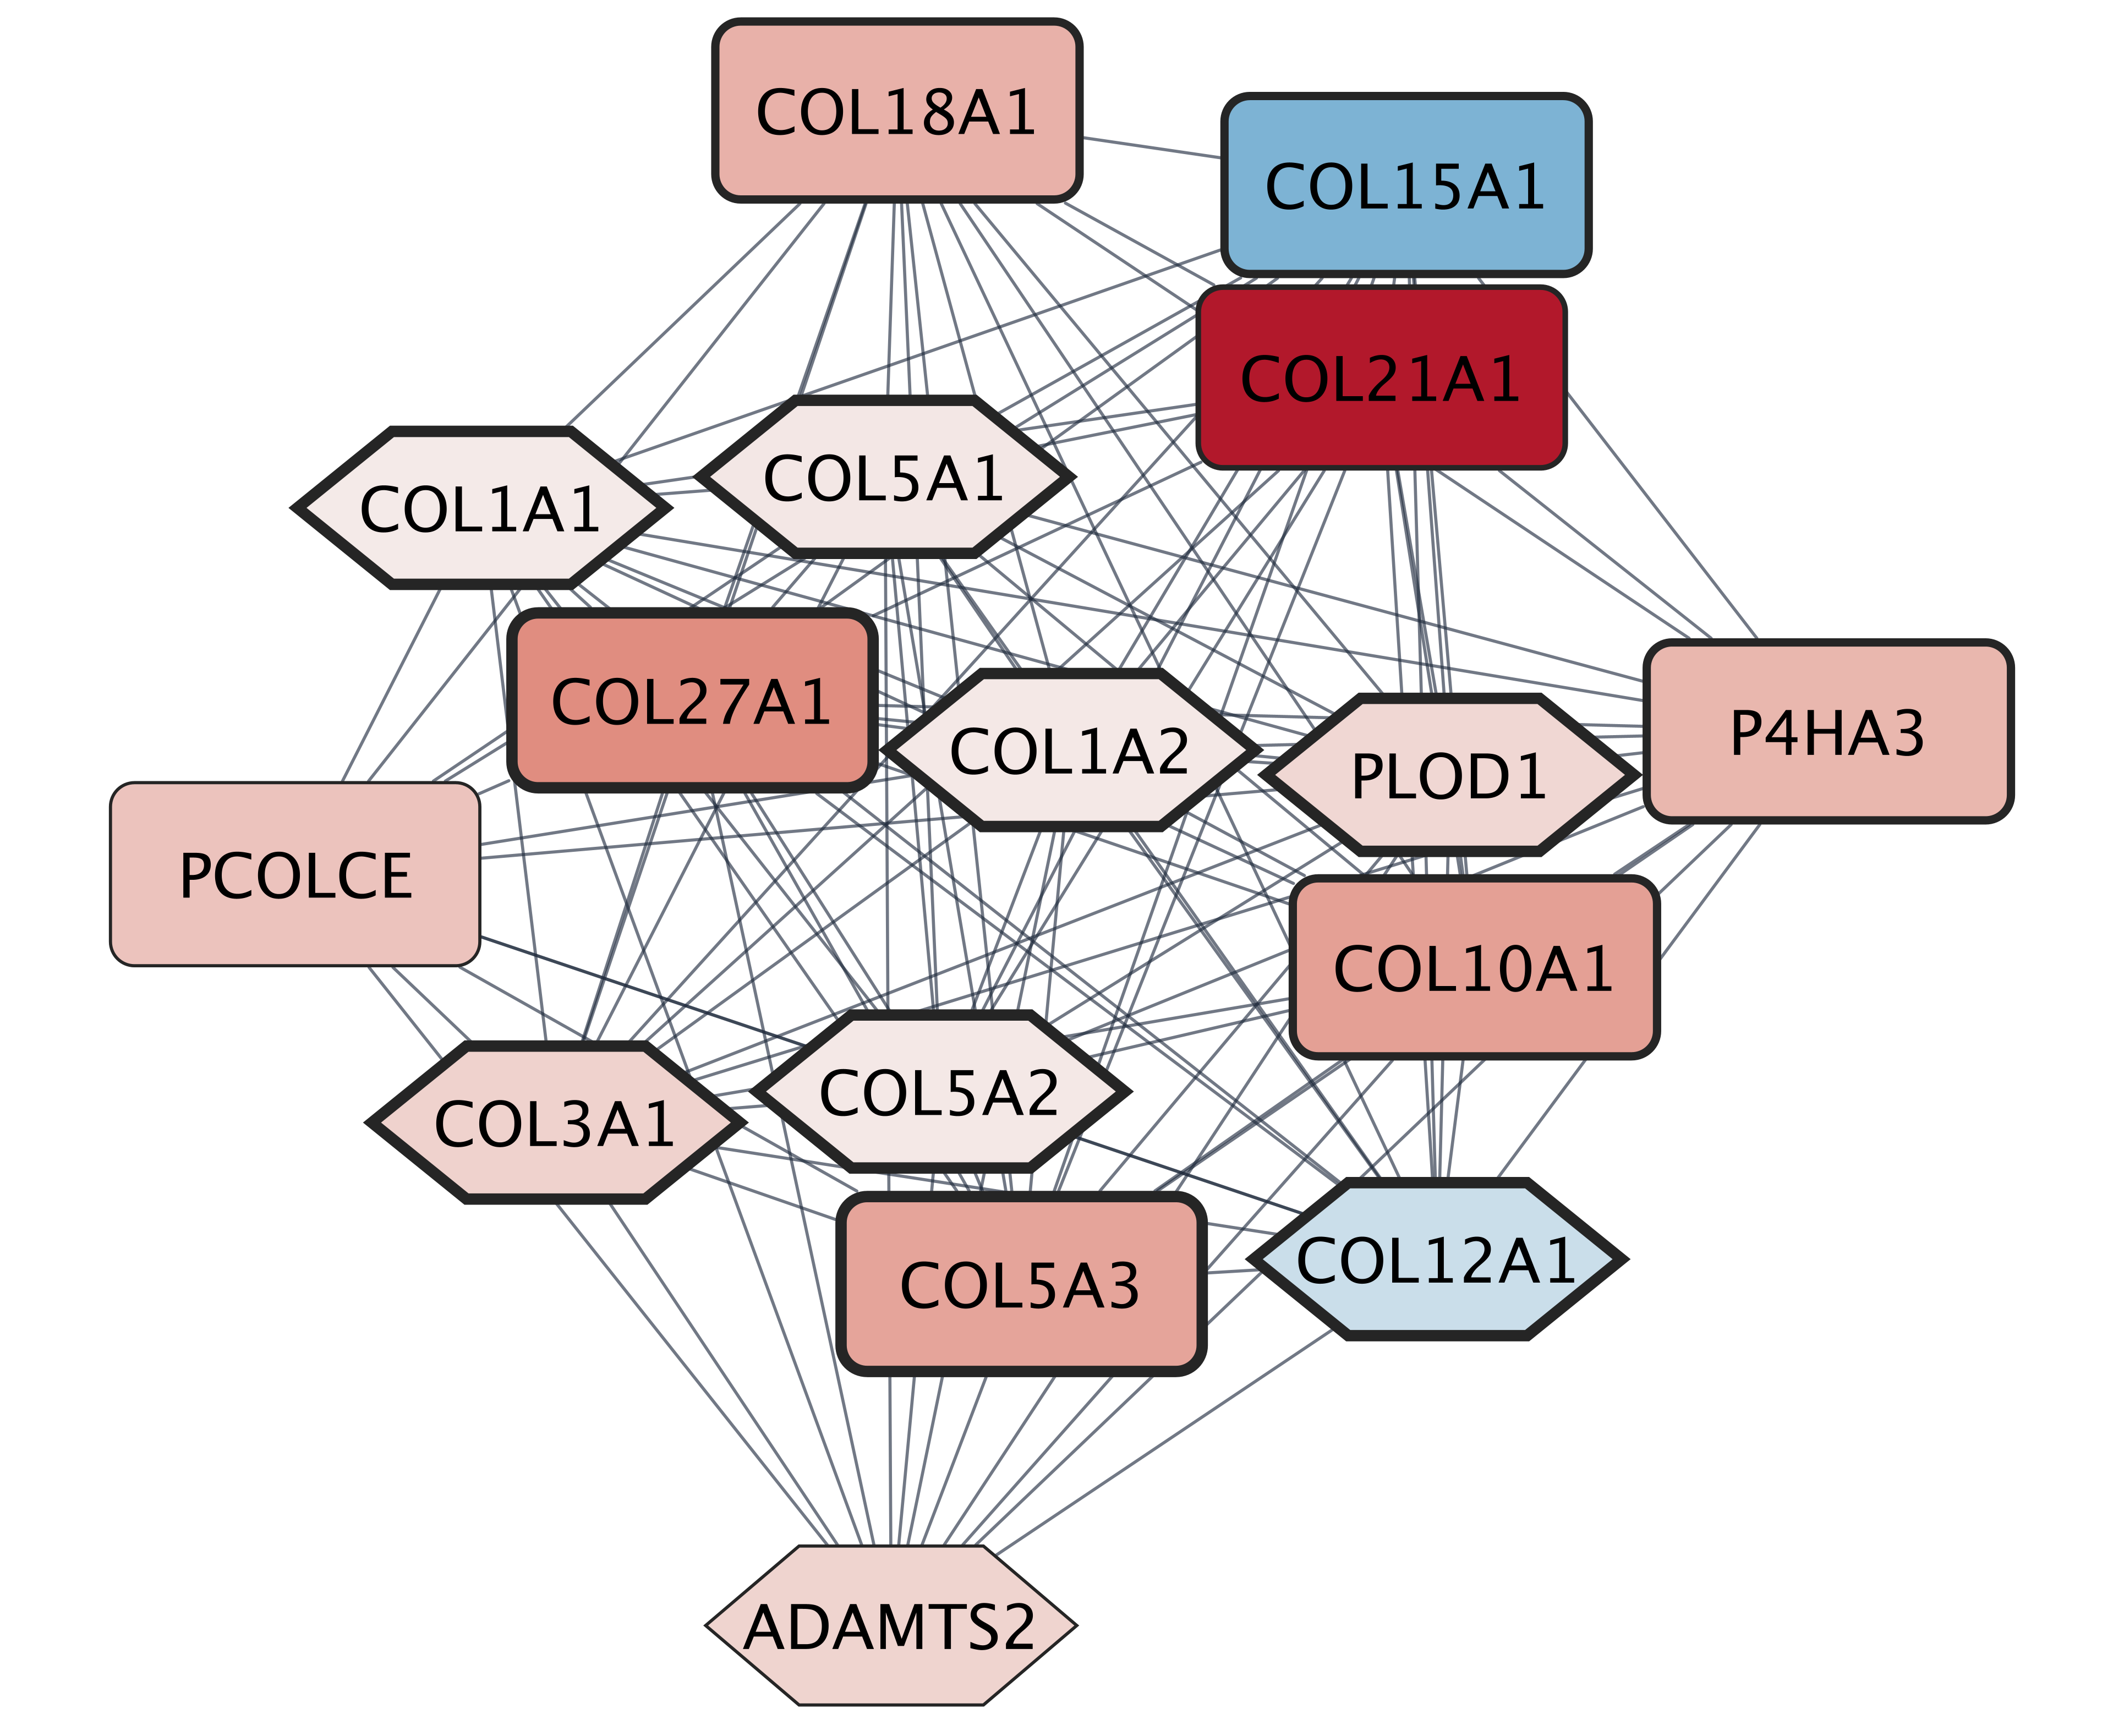
\includegraphics[width=\textwidth]{fig/mcode-cluster-without-enrichment.png}
 			\caption{Without visualization of the ECM GO term}
 	\end{subfigure}
 	\begin{subfigure}{.49\textwidth}
 		\centering
 		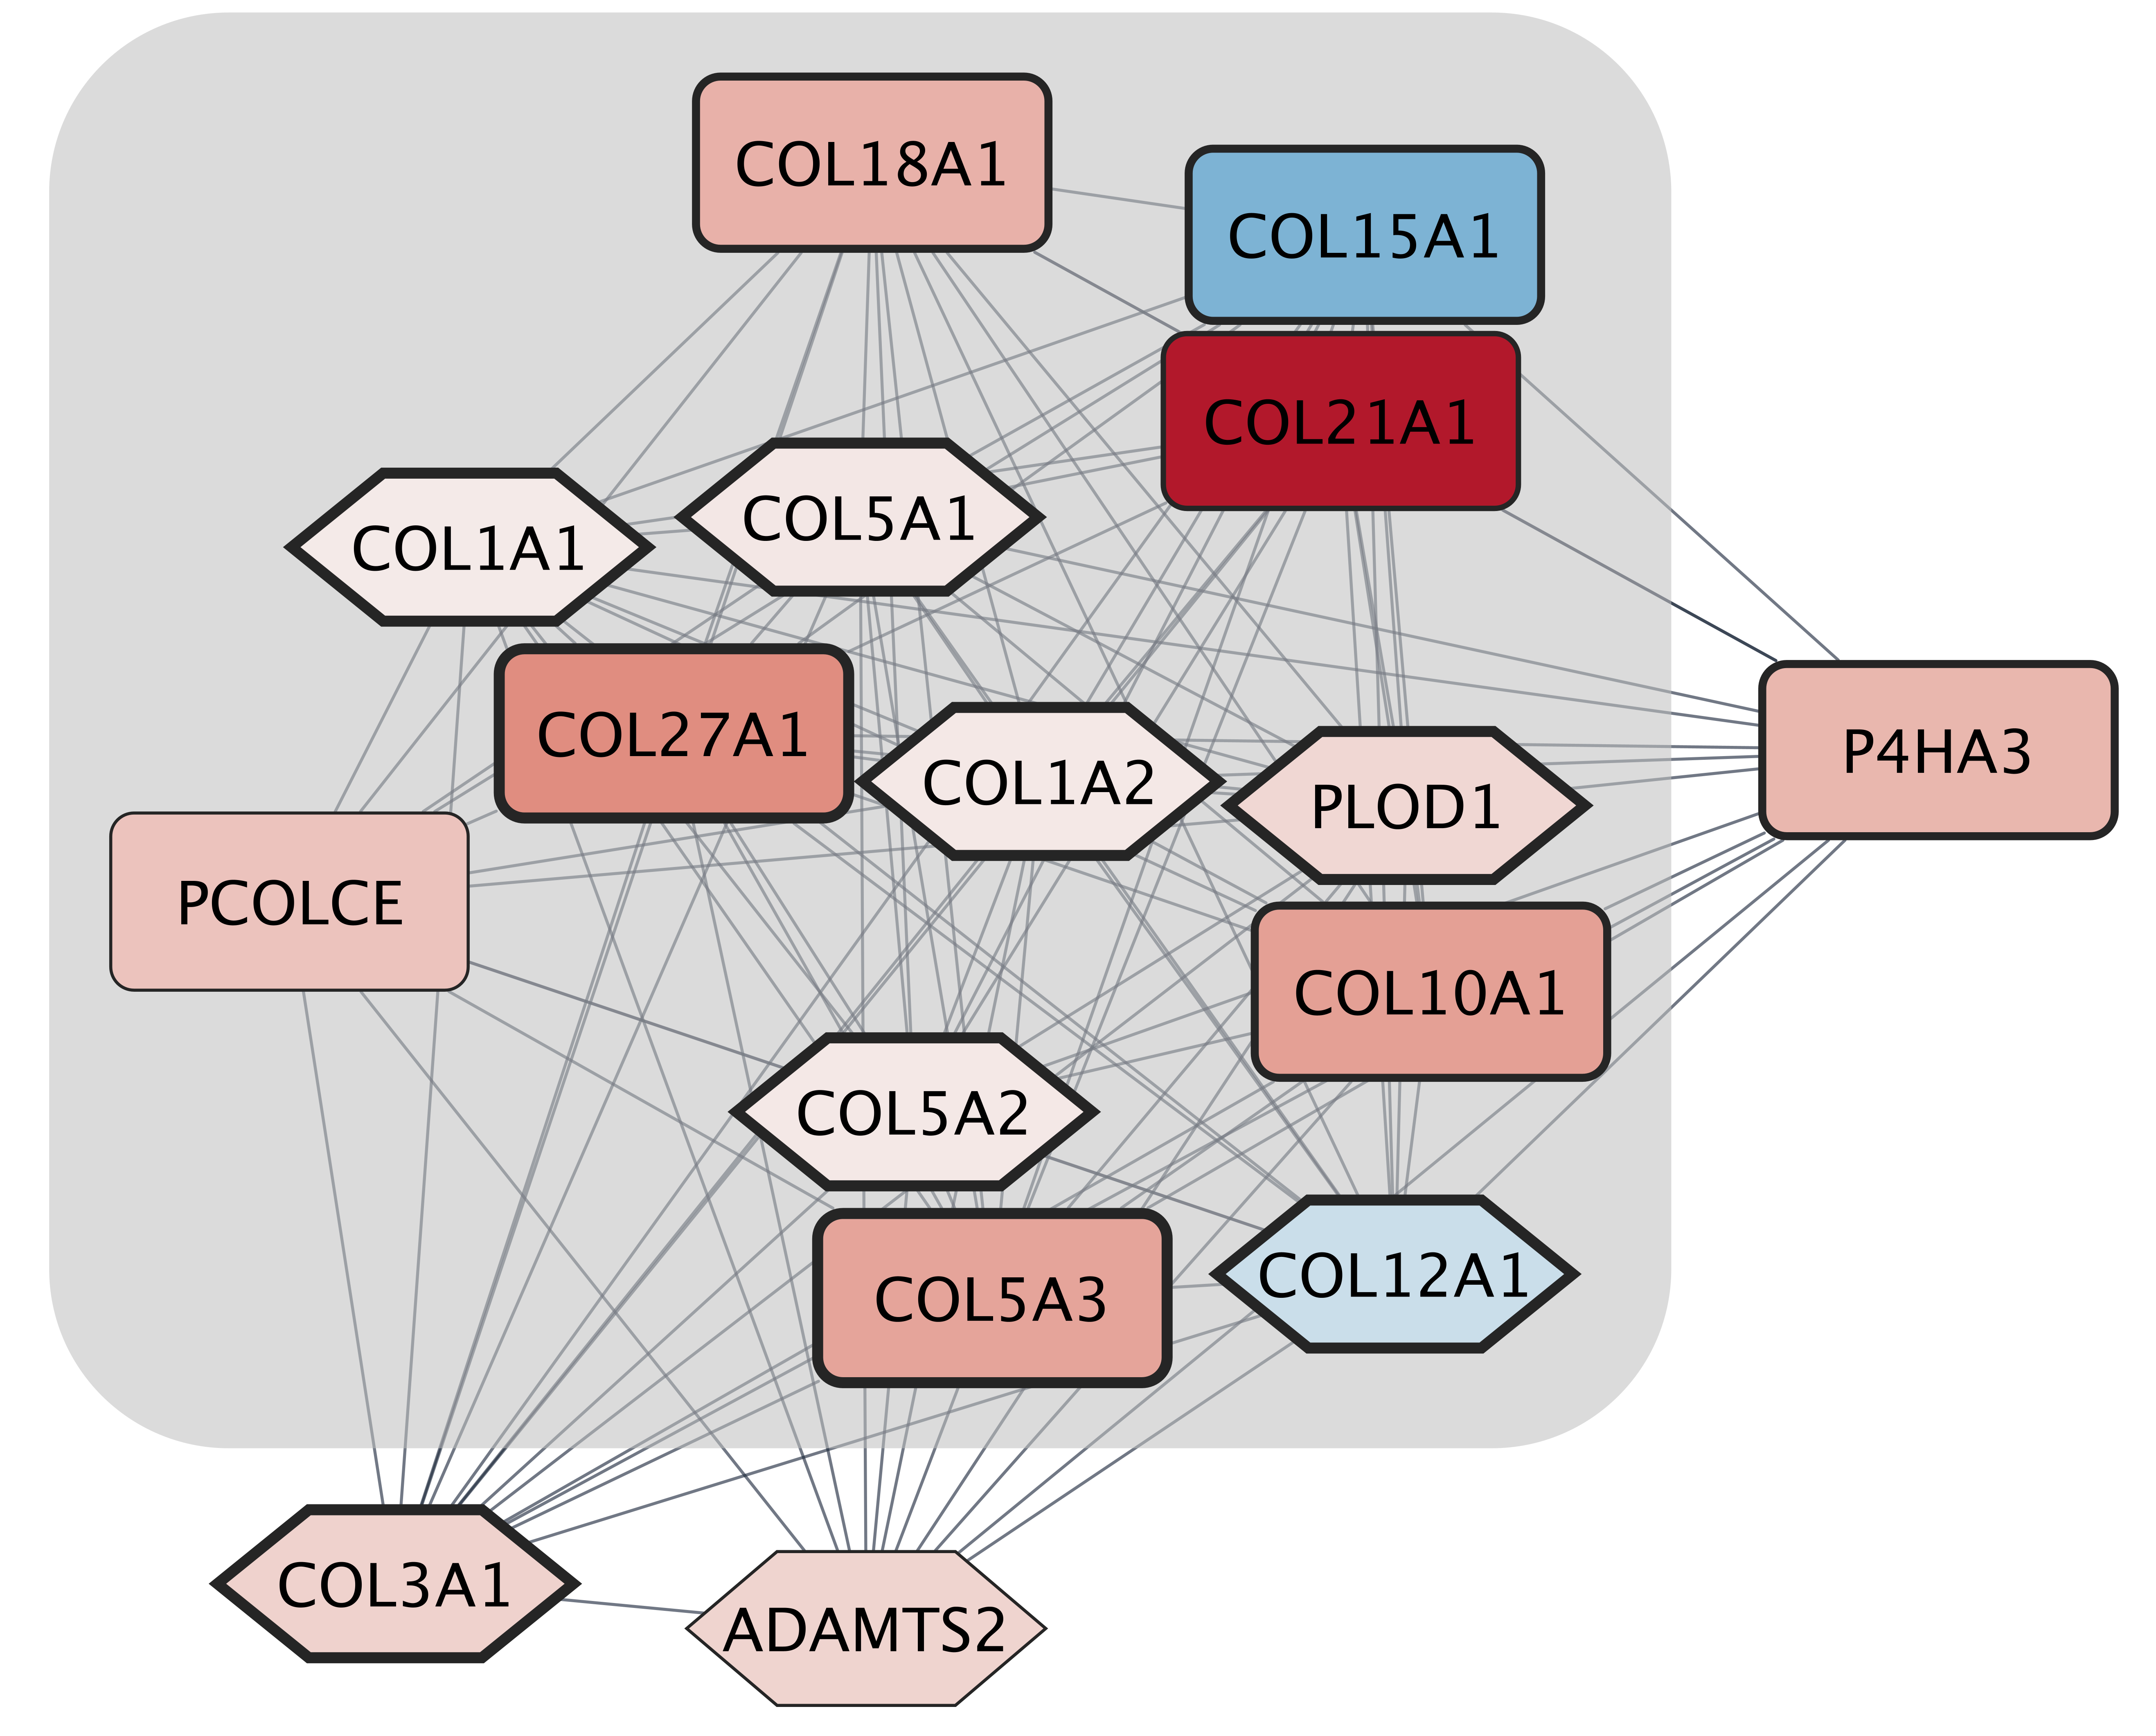
\includegraphics[width=\textwidth]{fig/mcode-cluster-eds-genes-with-ecm.png}
 		\caption{With visualization of the ECM GO term}
 	\end{subfigure}
	\caption[MCODE cluster with EDS genes]{\centering The MCODE cluster contains many genes known to cause other types of EDS. [TODO: add legend for shape, border and colour]}
	\label{fig:mcode3}
\end{figure}

GO-Enrichment testing overrepresentation of molecular functions of the cluster returns extracellular matrix in two terms, GO:0005201 and GO:0030020, with the second one being a subterm of the first. The first describes the action of a molecule that contributes to the structural integrity of the extracellular matrix; the second is a constituent of the extracellular matrix that enables the matrix to resist longitudinal stress. Both GO terms contain the same EDS genes and seven, respectively, six other genes, with PCOLE being the only gene not present in the GO subterm. These genes are investigated in more detail regarding their centrality, differential expression and what is known about them. COL27A1, a fibrillar collagen gene, has a central position in the cluster and relatively strong differential expression. The same applies to COL5A3, another gene related to collagen. The gene COL21A1 is very strongly differentially expressed, as mentioned before. It encodes the alpha chain of XXI collagen, which maintains the integrity of ECM and is a paralog to COL5A1, a known EDS gene \cite{COL21A1}.

To find connections to ECM in the enrichment analysis is consistent with findings of similar research \cite{Ritelli2022}. [Todo: there was other research, find] The affection of ECM with particular disorganisation of collagen and fibronecting was found in hEDS and two other EDS types \cite{Chiarelli2018}. [TODO: point out what my new findings are, COL21A1, etc.]

\paragraph{Up-regulated MCODE cluster}

The two larger, up-regulated MCODE clusters show no over-representation in ECM terms, as is shown in Figure \ref{fig:mcode-cluster-mf}. It is noticeable that the enrichment of the first cluster shows that only a few genes are part of the enriched terms. For the second cluster, the gene ratio is much higher, with up to around 80\,\% of the genes being involved in the second two terms. Therefore, the enrichment of the first cluster provides little insight into molecular function in hEDS patients.

 \begin{figure}[htb]
 	\centering
 	\caption*{\textbf{Molecular function enrichment for the two larger up-regulated clusters}}
		\begin{subfigure}{.49\textwidth}
			\centering
 			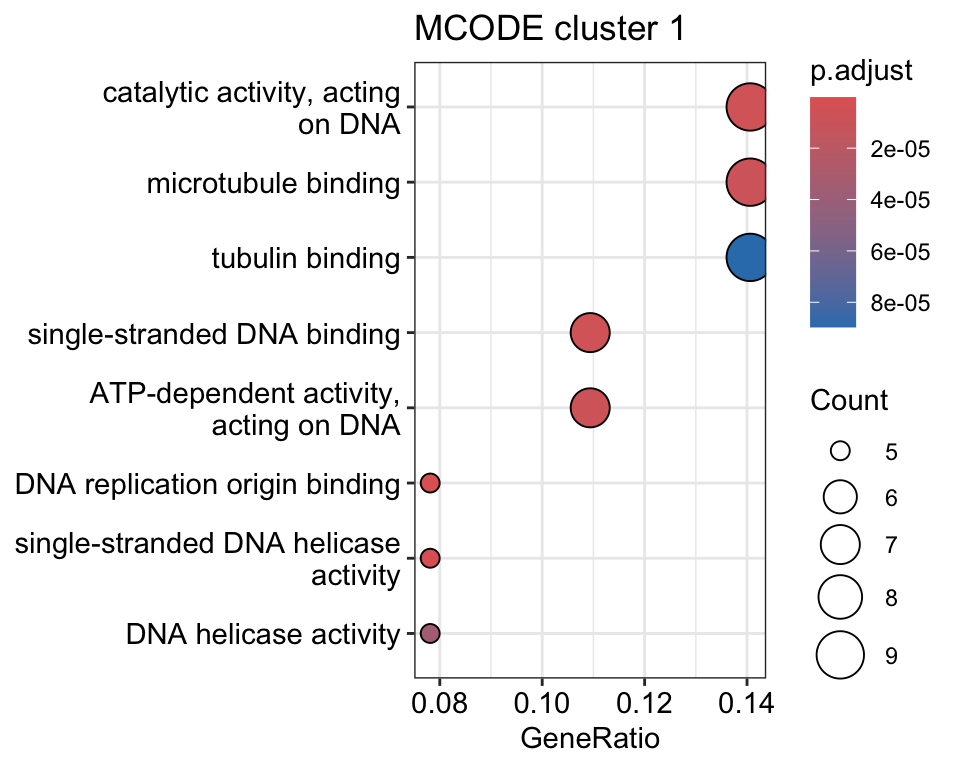
\includegraphics[width=\textwidth]{fig/mf-mcode-cluster1}
 			\caption{First MCODE cluster}
 		\end{subfigure}
    	\begin{subfigure}{.49\textwidth}
    		\centering
 			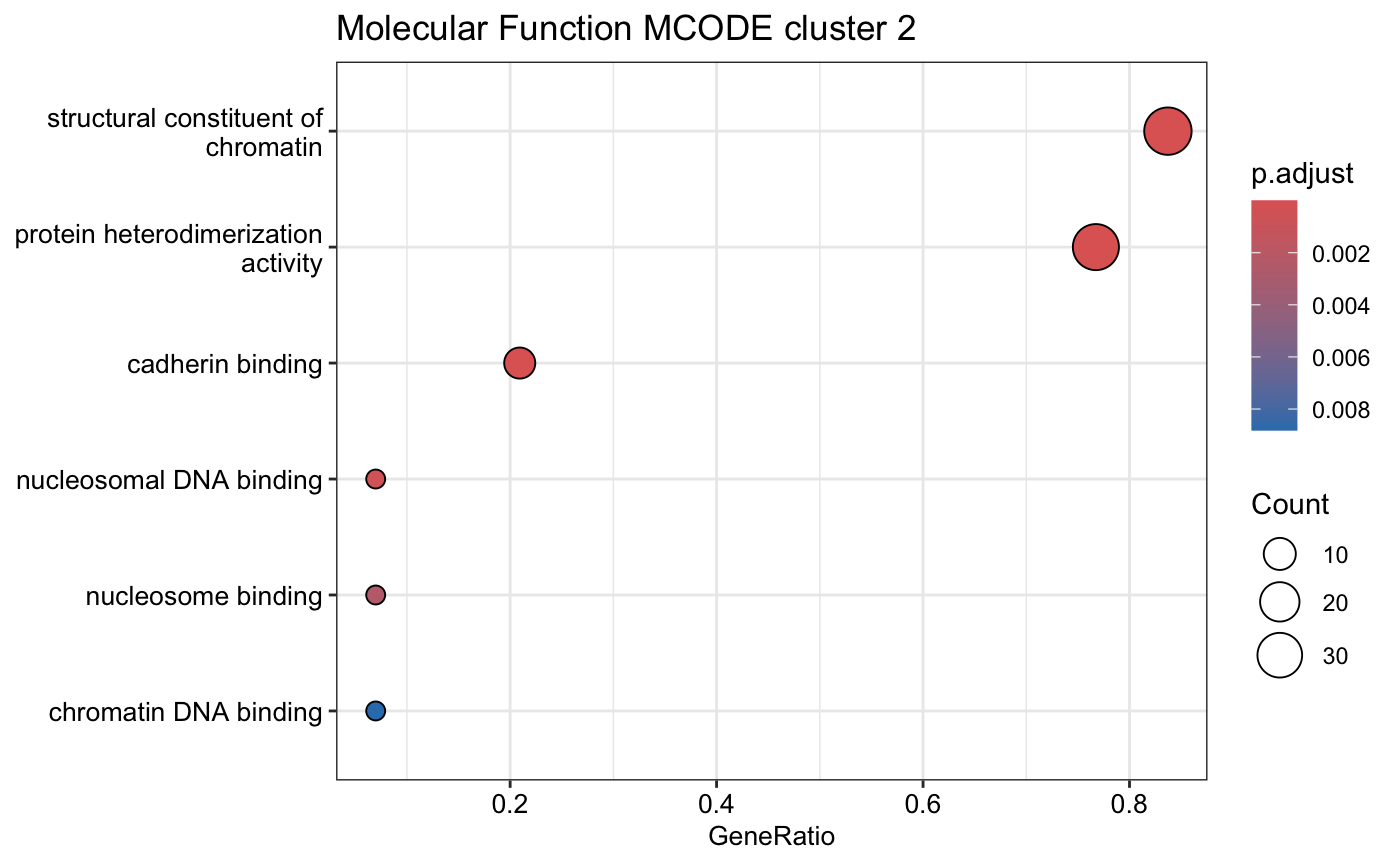
\includegraphics[width=\textwidth]{fig/mf-mcode-cluster2.png}
 			\caption{Second MCODE cluster}
 		\end{subfigure}
 	\caption{The results of the GO-enrichment for molecular function of the two up-regulated, larger MCODE clusters}
 	\label{fig:mcode-cluster-mf}
 \end{figure}

On the other hand, the up-regulation seen in the second cluster for the GO-term GO:0030527, the structural constituent of chromatin, is interesting because earlier research found down-regulated genes involved in processes related to chromatin in vEDS \cite{Chiarelli2018}.


\subsubsection{Community Clustering}

Community Clustering results in six clusters with more than 15 genes. Three are very small and loosely connected clusters, containing 18 to 29 genes and approximately the same amount of connections as genes. Since clusters of less than 20 genes are not large enough for analysis of biological processes, smaller clusters are omitted from the analysis. Additionally, there are two medium-sized highly connected clusters with 76 genes and 100 connections, and 105 genes and 2330 connections, respectively, and one huge cluster with 363 genes and 1661 connections.

\paragraph{Medium Sized Community Clusters}

The medium-sized clusters are highly interconnected and contain mainly up-regulated genes. Genes related to Nucleosome and protein-DNA complex are part of one of the clusters while the genes related to the chromosomal region are clustered in the other one.
\begin{itemize}
	\item first one: 5 highly differentielly expressed genes noticeable: H3C2, H3C7, H2BC10, ASF1B, WDR37
\end{itemize}


\paragraph{Largest Community Cluster}

The largest cluster contains a mix of up-regulated and down-regulated genes, and all 21 genes related to other EDS types. Furthermore, it contains all  genes being part of the GO-term for the ECM found in the over-representation of molecular functions of the MCODE cluster containing the EDS genes. The molecular cluster showing enrichment towards the chromatin part is not a part of this community cluster.

Heat Diffusion starting at EDS genes finds 39 DEG with a heat $> 0.1$ beside the starting nodes. These hot genes intersect with the MCODE cluster containing the EDS genes as it is expected due to their close connection reflected in the clustering. Beside those, there are 31 hot genes.

% CLEC3B, LAMA5, MAN1B1, PLS3, TNC (identified in paper), ADAMTS4, LAMB3, LAMB1, SLC4A11, MYLK, MKX, OGN, LOXL4, ASPN, MYH11, OLFML2B, COMP, C4B, HS6ST1 (identified in paper), FNDC1, INHBA, CHPF, LOXL1, GPC4, NUDCD1, ADAMTSL4, CSPG4, SULF1, NETO2 (identified in paper), CNIH3, ITGBL1

[TODO: check whether they were mentioned in other research and if we see them somewhere else]

\subsection{Discussion and Conclusion}

\begin{itemize}
	\item ECM/collagen in genes closely related to genes of other EDS types, seen in community cluster and MCODE cluster
	\item TODO: link to research, meaning
	\item chromatin related terms in a MCODE cluster and a community cluster found, in community cluster together with nucleosome
	\item chromatin interesting because down-regulated in other EDS type
	\item TODO: link to research, meaning
	\item heat diffusion in largest community cluster showed other genes additionally to ECM genes that are probably interesting
	\item project showed genes fullfilling similar roles than genes in other EDS types, candidates for causing hEDS
	\item hEDS has wide spectrum of representations, probably multiple components represented in the found clusters
\end{itemize}

% all chromatin genes in Community cluster 5